\documentclass[1p]{elsarticle_modified}
%\bibliographystyle{elsarticle-num}

%\usepackage[colorlinks]{hyperref}
%\usepackage{abbrmath_seonhwa} %\Abb, \Ascr, \Acal ,\Abf, \Afrak
\usepackage{amsfonts}
\usepackage{amssymb}
\usepackage{amsmath}
\usepackage{amsthm}
\usepackage{scalefnt}
\usepackage{amsbsy}
\usepackage{kotex}
\usepackage{caption}
\usepackage{subfig}
\usepackage{color}
\usepackage{graphicx}
\usepackage{xcolor} %% white, black, red, green, blue, cyan, magenta, yellow
\usepackage{float}
\usepackage{setspace}
\usepackage{hyperref}

\usepackage{tikz}
\usetikzlibrary{arrows}

\usepackage{multirow}
\usepackage{array} % fixed length table
\usepackage{hhline}

%%%%%%%%%%%%%%%%%%%%%
\makeatletter
\renewcommand*\env@matrix[1][\arraystretch]{%
	\edef\arraystretch{#1}%
	\hskip -\arraycolsep
	\let\@ifnextchar\new@ifnextchar
	\array{*\c@MaxMatrixCols c}}
\makeatother %https://tex.stackexchange.com/questions/14071/how-can-i-increase-the-line-spacing-in-a-matrix
%%%%%%%%%%%%%%%

\usepackage[normalem]{ulem}

\newcommand{\msout}[1]{\ifmmode\text{\sout{\ensuremath{#1}}}\else\sout{#1}\fi}
%SOURCE: \msout is \stkout macro in https://tex.stackexchange.com/questions/20609/strikeout-in-math-mode

\newcommand{\cancel}[1]{
	\ifmmode
	{\color{red}\msout{#1}}
	\else
	{\color{red}\sout{#1}}
	\fi
}

\newcommand{\add}[1]{
	{\color{blue}\uwave{#1}}
}

\newcommand{\replace}[2]{
	\ifmmode
	{\color{red}\msout{#1}}{\color{blue}\uwave{#2}}
	\else
	{\color{red}\sout{#1}}{\color{blue}\uwave{#2}}
	\fi
}

\newcommand{\Sol}{\mathcal{S}} %segment
\newcommand{\D}{D} %diagram
\newcommand{\A}{\mathcal{A}} %arc


%%%%%%%%%%%%%%%%%%%%%%%%%%%%%5 test

\def\sl{\operatorname{\textup{SL}}(2,\Cbb)}
\def\psl{\operatorname{\textup{PSL}}(2,\Cbb)}
\def\quan{\mkern 1mu \triangleright \mkern 1mu}

\theoremstyle{definition}
\newtheorem{thm}{Theorem}[section]
\newtheorem{prop}[thm]{Proposition}
\newtheorem{lem}[thm]{Lemma}
\newtheorem{ques}[thm]{Question}
\newtheorem{cor}[thm]{Corollary}
\newtheorem{defn}[thm]{Definition}
\newtheorem{exam}[thm]{Example}
\newtheorem{rmk}[thm]{Remark}
\newtheorem{alg}[thm]{Algorithm}

\newcommand{\I}{\sqrt{-1}}
\begin{document}

%\begin{frontmatter}
%
%\title{Boundary parabolic representations of knots up to 8 crossings}
%
%%% Group authors per affiliation:
%\author{Yunhi Cho} 
%\address{Department of Mathematics, University of Seoul, Seoul, Korea}
%\ead{yhcho@uos.ac.kr}
%
%
%\author{Seonhwa Kim} %\fnref{s_kim}}
%\address{Center for Geometry and Physics, Institute for Basic Science, Pohang, 37673, Korea}
%\ead{ryeona17@ibs.re.kr}
%
%\author{Hyuk Kim}
%\address{Department of Mathematical Sciences, Seoul National University, Seoul 08826, Korea}
%\ead{hyukkim@snu.ac.kr}
%
%\author{Seokbeom Yoon}
%\address{Department of Mathematical Sciences, Seoul National University, Seoul, 08826,  Korea}
%\ead{sbyoon15@snu.ac.kr}
%
%\begin{abstract}
%We find all boundary parabolic representation of knots up to 8 crossings.
%
%\end{abstract}
%\begin{keyword}
%    \MSC[2010] 57M25 
%\end{keyword}
%
%\end{frontmatter}

%\linenumbers
%\tableofcontents
%
\newcommand\colored[1]{\textcolor{white}{\rule[-0.35ex]{0.8em}{1.4ex}}\kern-0.8em\color{red} #1}%
%\newcommand\colored[1]{\textcolor{white}{ #1}\kern-2.17ex	\textcolor{white}{ #1}\kern-1.81ex	\textcolor{white}{ #1}\kern-2.15ex\color{red}#1	}

{\Large $\underline{12a_{1043}~(K12a_{1043})}$}

\setlength{\tabcolsep}{10pt}
\renewcommand{\arraystretch}{1.6}
\vspace{1cm}\begin{tabular}{m{100pt}>{\centering\arraybackslash}m{274pt}}
\multirow{5}{120pt}{
	\centering
	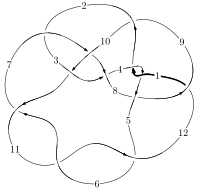
\includegraphics[width=112pt]{../../../GIT/diagram.site/Diagrams/png/1844_12a_1043.png}\\
\ \ \ A knot diagram\footnotemark}&
\allowdisplaybreaks
\textbf{Linearized knot diagam} \\
\cline{2-2}
 &
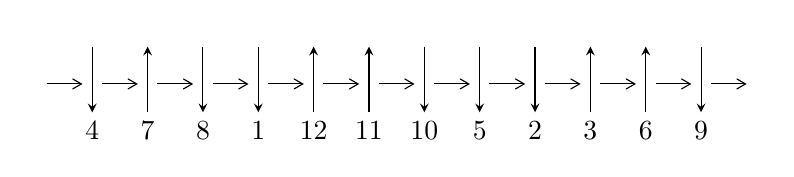
\begin{tikzpicture}[x=20pt, y=17pt]
	% nodes
	\node (C0) at (0, 0) {};
	\node (C1) at (1, 0) {};
	\node (C1U) at (1, +1) {};
	\node (C1D) at (1, -1) {4};

	\node (C2) at (2, 0) {};
	\node (C2U) at (2, +1) {};
	\node (C2D) at (2, -1) {7};

	\node (C3) at (3, 0) {};
	\node (C3U) at (3, +1) {};
	\node (C3D) at (3, -1) {8};

	\node (C4) at (4, 0) {};
	\node (C4U) at (4, +1) {};
	\node (C4D) at (4, -1) {1};

	\node (C5) at (5, 0) {};
	\node (C5U) at (5, +1) {};
	\node (C5D) at (5, -1) {12};

	\node (C6) at (6, 0) {};
	\node (C6U) at (6, +1) {};
	\node (C6D) at (6, -1) {11};

	\node (C7) at (7, 0) {};
	\node (C7U) at (7, +1) {};
	\node (C7D) at (7, -1) {10};

	\node (C8) at (8, 0) {};
	\node (C8U) at (8, +1) {};
	\node (C8D) at (8, -1) {5};

	\node (C9) at (9, 0) {};
	\node (C9U) at (9, +1) {};
	\node (C9D) at (9, -1) {2};

	\node (C10) at (10, 0) {};
	\node (C10U) at (10, +1) {};
	\node (C10D) at (10, -1) {3};

	\node (C11) at (11, 0) {};
	\node (C11U) at (11, +1) {};
	\node (C11D) at (11, -1) {6};

	\node (C12) at (12, 0) {};
	\node (C12U) at (12, +1) {};
	\node (C12D) at (12, -1) {9};
	\node (C13) at (13, 0) {};

	% arrows
	\draw[->,>={angle 60}]
	(C0) edge (C1) (C1) edge (C2) (C2) edge (C3) (C3) edge (C4) (C4) edge (C5) (C5) edge (C6) (C6) edge (C7) (C7) edge (C8) (C8) edge (C9) (C9) edge (C10) (C10) edge (C11) (C11) edge (C12) (C12) edge (C13) ;	\draw[->,>=stealth]
	(C1U) edge (C1D) (C2D) edge (C2U) (C3U) edge (C3D) (C4U) edge (C4D) (C5D) edge (C5U) (C6D) edge (C6U) (C7U) edge (C7D) (C8U) edge (C8D) (C9U) edge (C9D) (C10D) edge (C10U) (C11D) edge (C11U) (C12U) edge (C12D) ;
	\end{tikzpicture} \\
\hhline{~~} \\& 
\textbf{Solving Sequence} \\ \cline{2-2} 
 &
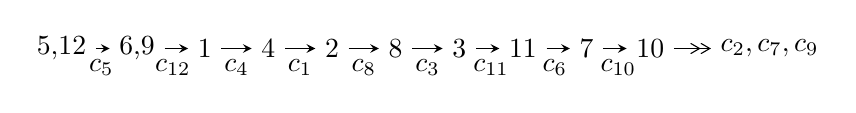
\begin{tikzpicture}[x=23pt, y=7pt]
	% node
	\node (A0) at (-1/8, 0) {5,12};
	\node (A1) at (17/16, 0) {6,9};
	\node (A2) at (17/8, 0) {1};
	\node (A3) at (25/8, 0) {4};
	\node (A4) at (33/8, 0) {2};
	\node (A5) at (41/8, 0) {8};
	\node (A6) at (49/8, 0) {3};
	\node (A7) at (57/8, 0) {11};
	\node (A8) at (65/8, 0) {7};
	\node (A9) at (73/8, 0) {10};
	\node (C1) at (1/2, -1) {$c_{5}$};
	\node (C2) at (13/8, -1) {$c_{12}$};
	\node (C3) at (21/8, -1) {$c_{4}$};
	\node (C4) at (29/8, -1) {$c_{1}$};
	\node (C5) at (37/8, -1) {$c_{8}$};
	\node (C6) at (45/8, -1) {$c_{3}$};
	\node (C7) at (53/8, -1) {$c_{11}$};
	\node (C8) at (61/8, -1) {$c_{6}$};
	\node (C9) at (69/8, -1) {$c_{10}$};
	\node (A10) at (11, 0) {$c_{2},c_{7},c_{9}$};

	% edge
	\draw[->,>=stealth]	
	(A0) edge (A1) (A1) edge (A2) (A2) edge (A3) (A3) edge (A4) (A4) edge (A5) (A5) edge (A6) (A6) edge (A7) (A7) edge (A8) (A8) edge (A9) ;
	\draw[->>,>={angle 60}]	
	(A9) edge (A10);
\end{tikzpicture} \\ 

\end{tabular} \\

\footnotetext{
The image of knot diagram is generated by the software ``\textbf{Draw programme}" developed by Andrew Bartholomew(\url{http://www.layer8.co.uk/maths/draw/index.htm\#Running-draw}), where we modified some parts for our purpose(\url{https://github.com/CATsTAILs/LinksPainter}).
}\phantom \\ \newline 
\centering \textbf{Ideals for irreducible components\footnotemark of $X_{\text{par}}$} 
 
\begin{align*}
I^u_{1}&=\langle 
309279332727 u^{39}-6570519786366 u^{38}+\cdots+25449616384 b-304514848348160,\\
\phantom{I^u_{1}}&\phantom{= \langle  }-446066672385 u^{39}+9504187459743 u^{38}+\cdots+25449616384 a+483336474422784,\\
\phantom{I^u_{1}}&\phantom{= \langle  }3 u^{40}-66 u^{39}+\cdots-43008 u+2048\rangle \\
I^u_{2}&=\langle 
1.99934\times10^{105} a^{21} u^{3}+1.76754\times10^{105} a^{20} u^{3}+\cdots+2.92106\times10^{102} a+2.33669\times10^{103},\\
\phantom{I^u_{2}}&\phantom{= \langle  }a^{21} u^3-5 a^{20} u^3+\cdots+24254 a-4243,\;u^4+u^3+3 u^2+2 u+1\rangle \\
I^u_{3}&=\langle 
1279125 u^{24}-1287228 u^{23}+\cdots+965461 b-3643883,\\
\phantom{I^u_{3}}&\phantom{= \langle  }10931649 u^{24}+12210774 u^{23}+\cdots+965461 a-9081154,\;3 u^{25}+3 u^{24}+\cdots-3 u+1\rangle \\
\\
\end{align*}
\raggedright * 3 irreducible components of $\dim_{\mathbb{C}}=0$, with total 153 representations.\\
\footnotetext{All coefficients of polynomials are rational numbers. But the coefficients are sometimes approximated in decimal forms when there is not enough margin.}
\newpage
\renewcommand{\arraystretch}{1}
\centering \section*{I. $I^u_{1}= \langle 3.09\times10^{11} u^{39}-6.57\times10^{12} u^{38}+\cdots+2.54\times10^{10} b-3.05\times10^{14},\;-4.46\times10^{11} u^{39}+9.50\times10^{12} u^{38}+\cdots+2.54\times10^{10} a+4.83\times10^{14},\;3 u^{40}-66 u^{39}+\cdots-43008 u+2048 \rangle$}
\flushleft \textbf{(i) Arc colorings}\\
\begin{tabular}{m{7pt} m{180pt} m{7pt} m{180pt} }
\flushright $a_{5}=$&$\begin{pmatrix}1\\0\end{pmatrix}$ \\
\flushright $a_{12}=$&$\begin{pmatrix}0\\u\end{pmatrix}$ \\
\flushright $a_{6}=$&$\begin{pmatrix}1\\- u^2\end{pmatrix}$ \\
\flushright $a_{9}=$&$\begin{pmatrix}17.5274 u^{39}-373.451 u^{38}+\cdots+369493. u-18991.9\\-12.1526 u^{39}+258.178 u^{38}+\cdots-232282. u+11965.4\end{pmatrix}$ \\
\flushright $a_{1}=$&$\begin{pmatrix}15.7231 u^{39}-330.923 u^{38}+\cdots+230269. u-11844.6\\-14.9846 u^{39}+317.152 u^{38}+\cdots-213560. u+10733.6\end{pmatrix}$ \\
\flushright $a_{4}=$&$\begin{pmatrix}17.7712 u^{39}-381.885 u^{38}+\cdots+379671. u-19416.9\\3.42698 u^{39}-69.4386 u^{38}+\cdots-31264.6 u+1902.33\end{pmatrix}$ \\
\flushright $a_{2}=$&$\begin{pmatrix}1.54086 u^{39}-32.5131 u^{38}+\cdots+7256.97 u-270.009\\5.16740 u^{39}-111.458 u^{38}+\cdots+131235. u-6838.08\end{pmatrix}$ \\
\flushright $a_{8}=$&$\begin{pmatrix}5.37483 u^{39}-115.274 u^{38}+\cdots+137212. u-7026.50\\-12.1526 u^{39}+258.178 u^{38}+\cdots-232282. u+11965.4\end{pmatrix}$ \\
\flushright $a_{3}=$&$\begin{pmatrix}11.4025 u^{39}-244.818 u^{38}+\cdots+259388. u-13416.8\\1.38575 u^{39}-29.6174 u^{38}+\cdots+21819.7 u-1051.89\end{pmatrix}$ \\
\flushright $a_{11}=$&$\begin{pmatrix}- u\\u^3+u\end{pmatrix}$ \\
\flushright $a_{7}=$&$\begin{pmatrix}u^2+1\\- u^4-2 u^2\end{pmatrix}$ \\
\flushright $a_{10}=$&$\begin{pmatrix}16.5400 u^{39}-352.658 u^{38}+\cdots+288678. u-14393.4\\-1.36215 u^{39}+27.8518 u^{38}+\cdots-32059.5 u+1831.54\end{pmatrix}$\\&\end{tabular}
\flushleft \textbf{(ii) Obstruction class $= -1$}\\~\\
\flushleft \textbf{(iii) Cusp Shapes $= \frac{10816413693}{6362404096} u^{39}-\frac{115564318683}{3181202048} u^{38}+\cdots+\frac{489218830366}{24853141} u-\frac{20767219470}{24853141}$}\\~\\
\newpage\renewcommand{\arraystretch}{1}
\flushleft \textbf{(iv) u-Polynomials at the component}\newline \\
\begin{tabular}{m{50pt}|m{274pt}}
Crossings & \hspace{64pt}u-Polynomials at each crossing \\
\hline $$\begin{aligned}c_{1},c_{4}\end{aligned}$$&$\begin{aligned}
&3(3 u^{40}-63 u^{39}+\cdots-4480 u+256)
\end{aligned}$\\
\hline $$\begin{aligned}c_{2},c_{10}\end{aligned}$$&$\begin{aligned}
&u^{40}+4 u^{38}+\cdots-3 u+3
\end{aligned}$\\
\hline $$\begin{aligned}c_{3},c_{9}\end{aligned}$$&$\begin{aligned}
&u^{40}-3 u^{39}+\cdots+10 u+25
\end{aligned}$\\
\hline $$\begin{aligned}c_{5},c_{6},c_{11}\end{aligned}$$&$\begin{aligned}
&3(3 u^{40}-66 u^{39}+\cdots-43008 u+2048)
\end{aligned}$\\
\hline $$\begin{aligned}c_{7}\end{aligned}$$&$\begin{aligned}
&3(3 u^{40}-90 u^{39}+\cdots-96 u+16)
\end{aligned}$\\
\hline $$\begin{aligned}c_{8},c_{12}\end{aligned}$$&$\begin{aligned}
&u^{40}+u^{39}+\cdots+36 u+9
\end{aligned}$\\
\hline
\end{tabular}\\~\\
\newpage\renewcommand{\arraystretch}{1}
\flushleft \textbf{(v) Riley Polynomials at the component}\newline \\
\begin{tabular}{m{50pt}|m{274pt}}
Crossings & \hspace{64pt}Riley Polynomials at each crossing \\
\hline $$\begin{aligned}c_{1},c_{4}\end{aligned}$$&$\begin{aligned}
&9(9 y^{40}+207 y^{39}+\cdots+876544 y+65536)
\end{aligned}$\\
\hline $$\begin{aligned}c_{2},c_{10}\end{aligned}$$&$\begin{aligned}
&y^{40}+8 y^{39}+\cdots-63 y+9
\end{aligned}$\\
\hline $$\begin{aligned}c_{3},c_{9}\end{aligned}$$&$\begin{aligned}
&y^{40}-19 y^{39}+\cdots-1150 y+625
\end{aligned}$\\
\hline $$\begin{aligned}c_{5},c_{6},c_{11}\end{aligned}$$&$\begin{aligned}
&9(9 y^{40}+306 y^{39}+\cdots+2097152 y+4194304)
\end{aligned}$\\
\hline $$\begin{aligned}c_{7}\end{aligned}$$&$\begin{aligned}
&9(9 y^{40}-36 y^{39}+\cdots-12928 y+256)
\end{aligned}$\\
\hline $$\begin{aligned}c_{8},c_{12}\end{aligned}$$&$\begin{aligned}
&y^{40}+y^{39}+\cdots+324 y+81
\end{aligned}$\\
\hline
\end{tabular}\\~\\
\newpage\flushleft \textbf{(vi) Complex Volumes and Cusp Shapes}
$$\begin{array}{c|c|c}  
\text{Solutions to }I^u_{1}& \I (\text{vol} + \sqrt{-1}CS) & \text{Cusp shape}\\
 \hline 
\begin{aligned}
u &= \phantom{-}0.430076 + 0.939129 I \\
a &= \phantom{-}0.709951 - 0.050908 I \\
b &= -0.353142 - 0.644841 I\end{aligned}
 & \phantom{-}2.91207 + 3.15877 I & \phantom{-0.000000 } 0 \\ \hline\begin{aligned}
u &= \phantom{-}0.430076 - 0.939129 I \\
a &= \phantom{-}0.709951 + 0.050908 I \\
b &= -0.353142 + 0.644841 I\end{aligned}
 & \phantom{-}2.91207 - 3.15877 I & \phantom{-0.000000 } 0 \\ \hline\begin{aligned}
u &= \phantom{-}0.231231 + 0.892892 I \\
a &= -0.389877 - 0.824893 I \\
b &= -0.646388 + 0.538859 I\end{aligned}
 & -0.74157 + 1.76866 I & \phantom{-0.000000 } 0 \\ \hline\begin{aligned}
u &= \phantom{-}0.231231 - 0.892892 I \\
a &= -0.389877 + 0.824893 I \\
b &= -0.646388 - 0.538859 I\end{aligned}
 & -0.74157 - 1.76866 I & \phantom{-0.000000 } 0 \\ \hline\begin{aligned}
u &= \phantom{-}0.797794 + 0.829732 I \\
a &= \phantom{-}0.079070 + 1.281020 I \\
b &= \phantom{-}0.99982 - 1.08760 I\end{aligned}
 & -0.4120 + 15.0532 I & \phantom{-0.000000 } 0 \\ \hline\begin{aligned}
u &= \phantom{-}0.797794 - 0.829732 I \\
a &= \phantom{-}0.079070 - 1.281020 I \\
b &= \phantom{-}0.99982 + 1.08760 I\end{aligned}
 & -0.4120 - 15.0532 I & \phantom{-0.000000 } 0 \\ \hline\begin{aligned}
u &= \phantom{-}1.143770 + 0.218983 I \\
a &= \phantom{-}0.669280 + 0.663411 I \\
b &= -0.620227 - 0.905352 I\end{aligned}
 & \phantom{-}1.46137 - 8.89771 I & \phantom{-0.000000 } 0 \\ \hline\begin{aligned}
u &= \phantom{-}1.143770 - 0.218983 I \\
a &= \phantom{-}0.669280 - 0.663411 I \\
b &= -0.620227 + 0.905352 I\end{aligned}
 & \phantom{-}1.46137 + 8.89771 I & \phantom{-0.000000 } 0 \\ \hline\begin{aligned}
u &= \phantom{-}1.061750 + 0.531482 I \\
a &= -0.592784 - 0.312411 I \\
b &= \phantom{-}0.463345 + 0.646754 I\end{aligned}
 & -0.374138 + 0.723530 I & \phantom{-0.000000 } 0 \\ \hline\begin{aligned}
u &= \phantom{-}1.061750 - 0.531482 I \\
a &= -0.592784 + 0.312411 I \\
b &= \phantom{-}0.463345 - 0.646754 I\end{aligned}
 & -0.374138 - 0.723530 I & \phantom{-0.000000 } 0\\
 \hline 
 \end{array}$$\newpage$$\begin{array}{c|c|c}  
\text{Solutions to }I^u_{1}& \I (\text{vol} + \sqrt{-1}CS) & \text{Cusp shape}\\
 \hline 
\begin{aligned}
u &= \phantom{-}0.366980 + 1.149690 I \\
a &= -0.587719 - 1.101030 I \\
b &= -1.05016 + 1.07975 I\end{aligned}
 & \phantom{-}1.86448 + 4.61004 I & \phantom{-0.000000 } 0 \\ \hline\begin{aligned}
u &= \phantom{-}0.366980 - 1.149690 I \\
a &= -0.587719 + 1.101030 I \\
b &= -1.05016 - 1.07975 I\end{aligned}
 & \phantom{-}1.86448 - 4.61004 I & \phantom{-0.000000 } 0 \\ \hline\begin{aligned}
u &= \phantom{-}0.962991 + 0.729062 I \\
a &= \phantom{-}0.057833 - 1.141700 I \\
b &= -0.888065 + 1.057290 I\end{aligned}
 & -0.88372 + 5.83229 I & \phantom{-0.000000 } 0 \\ \hline\begin{aligned}
u &= \phantom{-}0.962991 - 0.729062 I \\
a &= \phantom{-}0.057833 + 1.141700 I \\
b &= -0.888065 - 1.057290 I\end{aligned}
 & -0.88372 - 5.83229 I & \phantom{-0.000000 } 0 \\ \hline\begin{aligned}
u &= \phantom{-}0.895035 + 0.886441 I \\
a &= -0.165708 + 0.723991 I \\
b &= \phantom{-}0.790089 - 0.501107 I\end{aligned}
 & -4.31918 + 8.60646 I & \phantom{-0.000000 } 0 \\ \hline\begin{aligned}
u &= \phantom{-}0.895035 - 0.886441 I \\
a &= -0.165708 - 0.723991 I \\
b &= \phantom{-}0.790089 + 0.501107 I\end{aligned}
 & -4.31918 - 8.60646 I & \phantom{-0.000000 } 0 \\ \hline\begin{aligned}
u &= \phantom{-}0.714926 + 0.070491 I \\
a &= -0.80903 + 1.42994 I \\
b &= \phantom{-}0.679194 - 0.965270 I\end{aligned}
 & \phantom{-}5.53685 + 0.79423 I & \phantom{-0.000000 } 0 \\ \hline\begin{aligned}
u &= \phantom{-}0.714926 - 0.070491 I \\
a &= -0.80903 - 1.42994 I \\
b &= \phantom{-}0.679194 + 0.965270 I\end{aligned}
 & \phantom{-}5.53685 - 0.79423 I & \phantom{-0.000000 } 0 \\ \hline\begin{aligned}
u &= \phantom{-}0.434361 + 0.523139 I \\
a &= -0.45056 - 1.78531 I \\
b &= -0.738261 + 1.011170 I\end{aligned}
 & \phantom{-}1.76895 + 1.27338 I & \phantom{-0.000000 } 0. - 4.56377 I \\ \hline\begin{aligned}
u &= \phantom{-}0.434361 - 0.523139 I \\
a &= -0.45056 + 1.78531 I \\
b &= -0.738261 - 1.011170 I\end{aligned}
 & \phantom{-}1.76895 - 1.27338 I & \phantom{-0.000000 -}0. + 4.56377 I\\
 \hline 
 \end{array}$$\newpage$$\begin{array}{c|c|c}  
\text{Solutions to }I^u_{1}& \I (\text{vol} + \sqrt{-1}CS) & \text{Cusp shape}\\
 \hline 
\begin{aligned}
u &= \phantom{-}0.519767 + 0.325027 I \\
a &= -0.567043 - 0.806038 I \\
b &= \phantom{-}0.032746 + 0.603256 I\end{aligned}
 & \phantom{-}0.90033 + 1.11286 I & \phantom{-}3.57927 - 3.43616 I \\ \hline\begin{aligned}
u &= \phantom{-}0.519767 - 0.325027 I \\
a &= -0.567043 + 0.806038 I \\
b &= \phantom{-}0.032746 - 0.603256 I\end{aligned}
 & \phantom{-}0.90033 - 1.11286 I & \phantom{-}3.57927 + 3.43616 I \\ \hline\begin{aligned}
u &= \phantom{-}0.400531 + 0.362017 I \\
a &= -1.56564 - 0.64119 I \\
b &= \phantom{-}0.394968 + 0.823605 I\end{aligned}
 & \phantom{-}2.18207 + 1.75911 I & \phantom{-}3.60232 - 4.80724 I \\ \hline\begin{aligned}
u &= \phantom{-}0.400531 - 0.362017 I \\
a &= -1.56564 + 0.64119 I \\
b &= \phantom{-}0.394968 - 0.823605 I\end{aligned}
 & \phantom{-}2.18207 - 1.75911 I & \phantom{-}3.60232 + 4.80724 I \\ \hline\begin{aligned}
u &= \phantom{-}0.10737 + 1.52582 I \\
a &= \phantom{-}0.394221 + 0.366834 I \\
b &= \phantom{-}0.517395 - 0.640896 I\end{aligned}
 & -5.33866 + 3.18854 I & \phantom{-0.000000 } 0 \\ \hline\begin{aligned}
u &= \phantom{-}0.10737 - 1.52582 I \\
a &= \phantom{-}0.394221 - 0.366834 I \\
b &= \phantom{-}0.517395 + 0.640896 I\end{aligned}
 & -5.33866 - 3.18854 I & \phantom{-0.000000 } 0 \\ \hline\begin{aligned}
u &= \phantom{-}0.10832 + 1.54869 I \\
a &= \phantom{-}0.689279 + 0.757629 I \\
b &= \phantom{-}1.09867 - 1.14955 I\end{aligned}
 & -5.20346 + 3.15092 I & \phantom{-0.000000 } 0 \\ \hline\begin{aligned}
u &= \phantom{-}0.10832 - 1.54869 I \\
a &= \phantom{-}0.689279 - 0.757629 I \\
b &= \phantom{-}1.09867 + 1.14955 I\end{aligned}
 & -5.20346 - 3.15092 I & \phantom{-0.000000 } 0 \\ \hline\begin{aligned}
u &= \phantom{-}0.25142 + 1.65145 I \\
a &= -0.569813 - 0.870066 I \\
b &= -1.29361 + 1.15977 I\end{aligned}
 & -8.6562 + 19.0603 I & \phantom{-0.000000 } 0 \\ \hline\begin{aligned}
u &= \phantom{-}0.25142 - 1.65145 I \\
a &= -0.569813 + 0.870066 I \\
b &= -1.29361 - 1.15977 I\end{aligned}
 & -8.6562 - 19.0603 I & \phantom{-0.000000 } 0\\
 \hline 
 \end{array}$$\newpage$$\begin{array}{c|c|c}  
\text{Solutions to }I^u_{1}& \I (\text{vol} + \sqrt{-1}CS) & \text{Cusp shape}\\
 \hline 
\begin{aligned}
u &= \phantom{-}0.29257 + 1.65671 I \\
a &= \phantom{-}0.538073 + 0.853110 I \\
b &= \phantom{-}1.25593 - 1.14103 I\end{aligned}
 & -8.82937 + 10.53240 I & \phantom{-0.000000 } 0 \\ \hline\begin{aligned}
u &= \phantom{-}0.29257 - 1.65671 I \\
a &= \phantom{-}0.538073 - 0.853110 I \\
b &= \phantom{-}1.25593 + 1.14103 I\end{aligned}
 & -8.82937 - 10.53240 I & \phantom{-0.000000 } 0 \\ \hline\begin{aligned}
u &= \phantom{-}0.26892 + 1.66392 I \\
a &= -0.295163 - 0.749259 I \\
b &= -1.167330 + 0.692615 I\end{aligned}
 & -12.7100 + 12.9921 I & \phantom{-0.000000 } 0 \\ \hline\begin{aligned}
u &= \phantom{-}0.26892 - 1.66392 I \\
a &= -0.295163 + 0.749259 I \\
b &= -1.167330 - 0.692615 I\end{aligned}
 & -12.7100 - 12.9921 I & \phantom{-0.000000 } 0 \\ \hline\begin{aligned}
u &= \phantom{-}1.38555 + 0.97091 I \\
a &= \phantom{-}0.086799 - 0.325668 I \\
b &= -0.436459 + 0.366956 I\end{aligned}
 & -2.92234 - 0.70874 I & \phantom{-0.000000 } 0 \\ \hline\begin{aligned}
u &= \phantom{-}1.38555 - 0.97091 I \\
a &= \phantom{-}0.086799 + 0.325668 I \\
b &= -0.436459 - 0.366956 I\end{aligned}
 & -2.92234 + 0.70874 I & \phantom{-0.000000 } 0 \\ \hline\begin{aligned}
u &= \phantom{-}0.29238 + 1.71673 I \\
a &= \phantom{-}0.277808 + 0.672154 I \\
b &= \phantom{-}1.072680 - 0.673445 I\end{aligned}
 & -11.76900 + 4.97311 I & \phantom{-0.000000 } 0 \\ \hline\begin{aligned}
u &= \phantom{-}0.29238 - 1.71673 I \\
a &= \phantom{-}0.277808 - 0.672154 I \\
b &= \phantom{-}1.072680 + 0.673445 I\end{aligned}
 & -11.76900 - 4.97311 I & \phantom{-0.000000 } 0 \\ \hline\begin{aligned}
u &= \phantom{-}0.33425 + 1.71922 I \\
a &= -0.008980 - 0.357256 I \\
b &= -0.611201 + 0.134853 I\end{aligned}
 & -7.92682 + 6.50746 I & \phantom{-0.000000 } 0 \\ \hline\begin{aligned}
u &= \phantom{-}0.33425 - 1.71922 I \\
a &= -0.008980 + 0.357256 I \\
b &= -0.611201 - 0.134853 I\end{aligned}
 & -7.92682 - 6.50746 I & \phantom{-0.000000 } 0\\
 \hline 
 \end{array}$$\newpage\newpage\renewcommand{\arraystretch}{1}
\centering \section*{II. $I^u_{2}= \langle 2.00\times10^{105} a^{21} u^{3}+1.77\times10^{105} a^{20} u^{3}+\cdots+2.92\times10^{102} a+2.34\times10^{103},\;a^{21} u^3-5 a^{20} u^3+\cdots+24254 a-4243,\;u^4+u^3+3 u^2+2 u+1 \rangle$}
\flushleft \textbf{(i) Arc colorings}\\
\begin{tabular}{m{7pt} m{180pt} m{7pt} m{180pt} }
\flushright $a_{5}=$&$\begin{pmatrix}1\\0\end{pmatrix}$ \\
\flushright $a_{12}=$&$\begin{pmatrix}0\\u\end{pmatrix}$ \\
\flushright $a_{6}=$&$\begin{pmatrix}1\\- u^2\end{pmatrix}$ \\
\flushright $a_{9}=$&$\begin{pmatrix}a\\-78.5727 a^{21} u^{3}-69.4631 a^{20} u^{3}+\cdots-0.114796 a-0.918302\end{pmatrix}$ \\
\flushright $a_{1}=$&$\begin{pmatrix}- a^2 u\\-8.74081 a^{21} u^{3}-5.12626 a^{20} u^{3}+\cdots+0.385900 a-0.158208\end{pmatrix}$ \\
\flushright $a_{4}=$&$\begin{pmatrix}-1.89040 a^{21} u^{3}+4.17765 a^{20} u^{3}+\cdots-0.411276 a+1.19408\\-6.23246 a^{21} u^{3}-3.30996 a^{20} u^{3}+\cdots+0.0353917 a+0.000856252\end{pmatrix}$ \\
\flushright $a_{2}=$&$\begin{pmatrix}2.63867 a^{21} u^{3}+13.9877 a^{20} u^{3}+\cdots-0.685670 a+0.182322\\-40.5506 a^{21} u^{3}+7.86725 a^{20} u^{3}+\cdots+0.957810 a-0.211076\end{pmatrix}$ \\
\flushright $a_{8}=$&$\begin{pmatrix}-78.5727 a^{21} u^{3}-69.4631 a^{20} u^{3}+\cdots+0.885204 a-0.918302\\-78.5727 a^{21} u^{3}-69.4631 a^{20} u^{3}+\cdots-0.114796 a-0.918302\end{pmatrix}$ \\
\flushright $a_{3}=$&$\begin{pmatrix}-87.9371 a^{21} u^{3}-42.3152 a^{20} u^{3}+\cdots-0.483802 a+0.569188\\-101.333 a^{21} u^{3}-79.9473 a^{20} u^{3}+\cdots-0.395275 a-0.785595\end{pmatrix}$ \\
\flushright $a_{11}=$&$\begin{pmatrix}- u\\u^3+u\end{pmatrix}$ \\
\flushright $a_{7}=$&$\begin{pmatrix}u^2+1\\u^3+u^2+2 u+1\end{pmatrix}$ \\
\flushright $a_{10}=$&$\begin{pmatrix}-57.6236 a^{21} u^{3}-64.1783 a^{20} u^{3}+\cdots+1.49037 a+0.268510\\-22.6994 a^{21} u^{3}-62.7768 a^{20} u^{3}+\cdots-1.47511 a-0.286750\end{pmatrix}$\\&\end{tabular}
\flushleft \textbf{(ii) Obstruction class $= -1$}\\~\\
\flushleft \textbf{(iii) Cusp Shapes $= 139.745 a^{21} u^{3}+269.849 a^{20} u^{3}+\cdots+8.18196 a-11.5585$}\\~\\
\newpage\renewcommand{\arraystretch}{1}
\flushleft \textbf{(iv) u-Polynomials at the component}\newline \\
\begin{tabular}{m{50pt}|m{274pt}}
Crossings & \hspace{64pt}u-Polynomials at each crossing \\
\hline $$\begin{aligned}c_{1},c_{4}\end{aligned}$$&$\begin{aligned}
&(u^{11}+3 u^{10}+\cdots+2 u+1)^{8}
\end{aligned}$\\
\hline $$\begin{aligned}c_{2},c_{10}\end{aligned}$$&$\begin{aligned}
&u^{88}+3 u^{87}+\cdots+313760 u+32689
\end{aligned}$\\
\hline $$\begin{aligned}c_{3},c_{9}\end{aligned}$$&$\begin{aligned}
&u^{88}+u^{87}+\cdots+7015212 u+14269049
\end{aligned}$\\
\hline $$\begin{aligned}c_{5},c_{6},c_{11}\end{aligned}$$&$\begin{aligned}
&(u^4+u^3+3 u^2+2 u+1)^{22}
\end{aligned}$\\
\hline $$\begin{aligned}c_{7}\end{aligned}$$&$\begin{aligned}
&(u^{11}+5 u^{10}+12 u^9+15 u^8+8 u^7-4 u^6-8 u^5-3 u^4+3 u^3+3 u^2-1)^8
\end{aligned}$\\
\hline $$\begin{aligned}c_{8},c_{12}\end{aligned}$$&$\begin{aligned}
&u^{88}- u^{87}+\cdots-584 u+83
\end{aligned}$\\
\hline
\end{tabular}\\~\\
\newpage\renewcommand{\arraystretch}{1}
\flushleft \textbf{(v) Riley Polynomials at the component}\newline \\
\begin{tabular}{m{50pt}|m{274pt}}
Crossings & \hspace{64pt}Riley Polynomials at each crossing \\
\hline $$\begin{aligned}c_{1},c_{4}\end{aligned}$$&$\begin{aligned}
&(y^{11}+7 y^{10}+\cdots-6 y-1)^{8}
\end{aligned}$\\
\hline $$\begin{aligned}c_{2},c_{10}\end{aligned}$$&$\begin{aligned}
&y^{88}+35 y^{87}+\cdots+45878166472 y+1068570721
\end{aligned}$\\
\hline $$\begin{aligned}c_{3},c_{9}\end{aligned}$$&$\begin{aligned}
&y^{88}-41 y^{87}+\cdots-6370049061361272 y+203605759364401
\end{aligned}$\\
\hline $$\begin{aligned}c_{5},c_{6},c_{11}\end{aligned}$$&$\begin{aligned}
&(y^4+5 y^3+7 y^2+2 y+1)^{22}
\end{aligned}$\\
\hline $$\begin{aligned}c_{7}\end{aligned}$$&$\begin{aligned}
&(y^{11}- y^{10}+\cdots+6 y-1)^{8}
\end{aligned}$\\
\hline $$\begin{aligned}c_{8},c_{12}\end{aligned}$$&$\begin{aligned}
&y^{88}-21 y^{87}+\cdots-714888 y+6889
\end{aligned}$\\
\hline
\end{tabular}\\~\\
\newpage\flushleft \textbf{(vi) Complex Volumes and Cusp Shapes}
$$\begin{array}{c|c|c}  
\text{Solutions to }I^u_{2}& \I (\text{vol} + \sqrt{-1}CS) & \text{Cusp shape}\\
 \hline 
\begin{aligned}
u &= -0.395123 + 0.506844 I \\
a &= \phantom{-}0.907790 + 0.226548 I \\
b &= -0.647304 + 1.109790 I\end{aligned}
 & \phantom{-}3.19680 + 3.58563 I & \phantom{-}3.66733 - 1.31877 I \\ \hline\begin{aligned}
u &= -0.395123 + 0.506844 I \\
a &= -0.017246 - 0.753773 I \\
b &= -1.163050 + 0.611843 I\end{aligned}
 & -2.23683 + 1.28930 I & -7.64088 + 4.99207 I \\ \hline\begin{aligned}
u &= -0.395123 + 0.506844 I \\
a &= \phantom{-}1.277480 + 0.112709 I \\
b &= -0.886862 + 0.535701 I\end{aligned}
 & \phantom{-}0.32630 + 4.50932 I & -7.34372 - 5.11480 I \\ \hline\begin{aligned}
u &= -0.395123 + 0.506844 I \\
a &= \phantom{-}0.578173 + 1.190000 I \\
b &= -0.944476 - 0.408288 I\end{aligned}
 & -3.81269 - 1.41510 I & -16.4346 + 4.9087 I \\ \hline\begin{aligned}
u &= -0.395123 + 0.506844 I \\
a &= -0.281884 + 0.537705 I \\
b &= \phantom{-}1.71358 - 1.04898 I\end{aligned}
 & -1.29627 - 6.63139 I & -4.6093 + 13.9215 I \\ \hline\begin{aligned}
u &= -0.395123 + 0.506844 I \\
a &= -0.72321 - 1.21563 I \\
b &= \phantom{-}0.189954 - 0.056607 I\end{aligned}
 & -1.85793 + 0.83268 I & -7.80908 - 0.15485 I \\ \hline\begin{aligned}
u &= -0.395123 + 0.506844 I \\
a &= \phantom{-}0.43939 + 1.37682 I \\
b &= -0.568100 - 0.987543 I\end{aligned}
 & -1.85793 - 3.66289 I & -7.80908 + 9.97234 I \\ \hline\begin{aligned}
u &= -0.395123 + 0.506844 I \\
a &= \phantom{-}0.53617 + 1.38915 I \\
b &= \phantom{-}0.292755 - 1.302630 I\end{aligned}
 & -2.23683 - 4.11951 I & -7.64088 + 4.82542 I \\ \hline\begin{aligned}
u &= -0.395123 + 0.506844 I \\
a &= \phantom{-}0.40425 - 1.54629 I \\
b &= \phantom{-}1.31383 + 1.13328 I\end{aligned}
 & \phantom{-}3.19680 - 6.41584 I & \phantom{-}3.66733 + 11.13625 I \\ \hline\begin{aligned}
u &= -0.395123 + 0.506844 I \\
a &= -0.40252 - 1.54965 I \\
b &= \phantom{-}0.831592 + 0.177152 I\end{aligned}
 & -3.81269 - 1.41510 I & -16.4346 + 4.9087 I\\
 \hline 
 \end{array}$$\newpage$$\begin{array}{c|c|c}  
\text{Solutions to }I^u_{2}& \I (\text{vol} + \sqrt{-1}CS) & \text{Cusp shape}\\
 \hline 
\begin{aligned}
u &= -0.395123 + 0.506844 I \\
a &= -1.50585 - 0.57585 I \\
b &= \phantom{-}0.561889 - 0.602950 I\end{aligned}
 & \phantom{-}0.32630 + 4.50932 I & -7.34372 - 5.11480 I \\ \hline\begin{aligned}
u &= -0.395123 + 0.506844 I \\
a &= \phantom{-}0.251194 + 0.178954 I \\
b &= -0.901890 - 0.113767 I\end{aligned}
 & -1.85793 + 0.83268 I & -7.80908 - 0.15485 I \\ \hline\begin{aligned}
u &= -0.395123 + 0.506844 I \\
a &= \phantom{-}0.66841 - 1.64193 I \\
b &= \phantom{-}0.871448 + 0.321314 I\end{aligned}
 & -1.85793 - 3.66289 I & -7.80908 + 9.97234 I \\ \hline\begin{aligned}
u &= -0.395123 + 0.506844 I \\
a &= -1.81056 + 0.60810 I \\
b &= -1.292500 - 0.105875 I\end{aligned}
 & -1.29627 + 3.80118 I & \phantom{-0.000000 } 0 \\ \hline\begin{aligned}
u &= -0.395123 + 0.506844 I \\
a &= -1.98119 + 0.26736 I \\
b &= \phantom{-}0.473513 - 0.370593 I\end{aligned}
 & \phantom{-}3.19680 + 3.58563 I & \phantom{-0.000000 } 0 \\ \hline\begin{aligned}
u &= -0.395123 + 0.506844 I \\
a &= -1.10659 - 1.68743 I \\
b &= -0.407184 + 1.157940 I\end{aligned}
 & -1.29627 + 3.80118 I & \phantom{-0.000000 } 0 \\ \hline\begin{aligned}
u &= -0.395123 + 0.506844 I \\
a &= -1.86351 - 0.84193 I \\
b &= -0.388860 - 0.289092 I\end{aligned}
 & -2.23683 + 1.28930 I & \phantom{-0.000000 } 0 \\ \hline\begin{aligned}
u &= -0.395123 + 0.506844 I \\
a &= \phantom{-}0.08448 + 2.04846 I \\
b &= -0.924867 - 1.064220 I\end{aligned}
 & \phantom{-}0.32630 - 7.33953 I & \phantom{-0.000000 } 0 \\ \hline\begin{aligned}
u &= -0.395123 + 0.506844 I \\
a &= \phantom{-}1.87864 - 0.88694 I \\
b &= \phantom{-}0.915937 + 0.277129 I\end{aligned}
 & -2.23683 - 4.11951 I & \phantom{-0.000000 } 0 \\ \hline\begin{aligned}
u &= -0.395123 + 0.506844 I \\
a &= \phantom{-}0.42118 - 2.15310 I \\
b &= \phantom{-}1.071630 + 0.766574 I\end{aligned}
 & \phantom{-}0.32630 - 7.33953 I & \phantom{-0.000000 } 0\\
 \hline 
 \end{array}$$\newpage$$\begin{array}{c|c|c}  
\text{Solutions to }I^u_{2}& \I (\text{vol} + \sqrt{-1}CS) & \text{Cusp shape}\\
 \hline 
\begin{aligned}
u &= -0.395123 + 0.506844 I \\
a &= -0.13382 + 2.69650 I \\
b &= -0.624000 - 0.815866 I\end{aligned}
 & \phantom{-}3.19680 - 6.41584 I & \phantom{-0.000000 } 0 \\ \hline\begin{aligned}
u &= -0.395123 + 0.506844 I \\
a &= \phantom{-}2.92664 + 1.09934 I \\
b &= \phantom{-}0.161153 + 0.355331 I\end{aligned}
 & -1.29627 - 6.63139 I & \phantom{-0.000000 } 0 \\ \hline\begin{aligned}
u &= -0.395123 - 0.506844 I \\
a &= \phantom{-}0.907790 - 0.226548 I \\
b &= -0.647304 - 1.109790 I\end{aligned}
 & \phantom{-}3.19680 - 3.58563 I & \phantom{-}3.66733 + 1.31877 I \\ \hline\begin{aligned}
u &= -0.395123 - 0.506844 I \\
a &= -0.017246 + 0.753773 I \\
b &= -1.163050 - 0.611843 I\end{aligned}
 & -2.23683 - 1.28930 I & -7.64088 - 4.99207 I \\ \hline\begin{aligned}
u &= -0.395123 - 0.506844 I \\
a &= \phantom{-}1.277480 - 0.112709 I \\
b &= -0.886862 - 0.535701 I\end{aligned}
 & \phantom{-}0.32630 - 4.50932 I & -7.34372 + 5.11480 I \\ \hline\begin{aligned}
u &= -0.395123 - 0.506844 I \\
a &= \phantom{-}0.578173 - 1.190000 I \\
b &= -0.944476 + 0.408288 I\end{aligned}
 & -3.81269 + 1.41510 I & -16.4346 - 4.9087 I \\ \hline\begin{aligned}
u &= -0.395123 - 0.506844 I \\
a &= -0.281884 - 0.537705 I \\
b &= \phantom{-}1.71358 + 1.04898 I\end{aligned}
 & -1.29627 + 6.63139 I & -4.6093 - 13.9215 I \\ \hline\begin{aligned}
u &= -0.395123 - 0.506844 I \\
a &= -0.72321 + 1.21563 I \\
b &= \phantom{-}0.189954 + 0.056607 I\end{aligned}
 & -1.85793 - 0.83268 I & -7.80908 + 0.15485 I \\ \hline\begin{aligned}
u &= -0.395123 - 0.506844 I \\
a &= \phantom{-}0.43939 - 1.37682 I \\
b &= -0.568100 + 0.987543 I\end{aligned}
 & -1.85793 + 3.66289 I & -7.80908 - 9.97234 I \\ \hline\begin{aligned}
u &= -0.395123 - 0.506844 I \\
a &= \phantom{-}0.53617 - 1.38915 I \\
b &= \phantom{-}0.292755 + 1.302630 I\end{aligned}
 & -2.23683 + 4.11951 I & -7.64088 - 4.82542 I\\
 \hline 
 \end{array}$$\newpage$$\begin{array}{c|c|c}  
\text{Solutions to }I^u_{2}& \I (\text{vol} + \sqrt{-1}CS) & \text{Cusp shape}\\
 \hline 
\begin{aligned}
u &= -0.395123 - 0.506844 I \\
a &= \phantom{-}0.40425 + 1.54629 I \\
b &= \phantom{-}1.31383 - 1.13328 I\end{aligned}
 & \phantom{-}3.19680 + 6.41584 I & \phantom{-}3.66733 - 11.13625 I \\ \hline\begin{aligned}
u &= -0.395123 - 0.506844 I \\
a &= -0.40252 + 1.54965 I \\
b &= \phantom{-}0.831592 - 0.177152 I\end{aligned}
 & -3.81269 + 1.41510 I & -16.4346 - 4.9087 I \\ \hline\begin{aligned}
u &= -0.395123 - 0.506844 I \\
a &= -1.50585 + 0.57585 I \\
b &= \phantom{-}0.561889 + 0.602950 I\end{aligned}
 & \phantom{-}0.32630 - 4.50932 I & -7.34372 + 5.11480 I \\ \hline\begin{aligned}
u &= -0.395123 - 0.506844 I \\
a &= \phantom{-}0.251194 - 0.178954 I \\
b &= -0.901890 + 0.113767 I\end{aligned}
 & -1.85793 - 0.83268 I & -7.80908 + 0.15485 I \\ \hline\begin{aligned}
u &= -0.395123 - 0.506844 I \\
a &= \phantom{-}0.66841 + 1.64193 I \\
b &= \phantom{-}0.871448 - 0.321314 I\end{aligned}
 & -1.85793 + 3.66289 I & -7.80908 - 9.97234 I \\ \hline\begin{aligned}
u &= -0.395123 - 0.506844 I \\
a &= -1.81056 - 0.60810 I \\
b &= -1.292500 + 0.105875 I\end{aligned}
 & -1.29627 - 3.80118 I & \phantom{-0.000000 } 0 \\ \hline\begin{aligned}
u &= -0.395123 - 0.506844 I \\
a &= -1.98119 - 0.26736 I \\
b &= \phantom{-}0.473513 + 0.370593 I\end{aligned}
 & \phantom{-}3.19680 - 3.58563 I & \phantom{-0.000000 } 0 \\ \hline\begin{aligned}
u &= -0.395123 - 0.506844 I \\
a &= -1.10659 + 1.68743 I \\
b &= -0.407184 - 1.157940 I\end{aligned}
 & -1.29627 - 3.80118 I & \phantom{-0.000000 } 0 \\ \hline\begin{aligned}
u &= -0.395123 - 0.506844 I \\
a &= -1.86351 + 0.84193 I \\
b &= -0.388860 + 0.289092 I\end{aligned}
 & -2.23683 - 1.28930 I & \phantom{-0.000000 } 0 \\ \hline\begin{aligned}
u &= -0.395123 - 0.506844 I \\
a &= \phantom{-}0.08448 - 2.04846 I \\
b &= -0.924867 + 1.064220 I\end{aligned}
 & \phantom{-}0.32630 + 7.33953 I & \phantom{-0.000000 } 0\\
 \hline 
 \end{array}$$\newpage$$\begin{array}{c|c|c}  
\text{Solutions to }I^u_{2}& \I (\text{vol} + \sqrt{-1}CS) & \text{Cusp shape}\\
 \hline 
\begin{aligned}
u &= -0.395123 - 0.506844 I \\
a &= \phantom{-}1.87864 + 0.88694 I \\
b &= \phantom{-}0.915937 - 0.277129 I\end{aligned}
 & -2.23683 + 4.11951 I & \phantom{-0.000000 } 0 \\ \hline\begin{aligned}
u &= -0.395123 - 0.506844 I \\
a &= \phantom{-}0.42118 + 2.15310 I \\
b &= \phantom{-}1.071630 - 0.766574 I\end{aligned}
 & \phantom{-}0.32630 + 7.33953 I & \phantom{-0.000000 } 0 \\ \hline\begin{aligned}
u &= -0.395123 - 0.506844 I \\
a &= -0.13382 - 2.69650 I \\
b &= -0.624000 + 0.815866 I\end{aligned}
 & \phantom{-}3.19680 + 6.41584 I & \phantom{-0.000000 } 0 \\ \hline\begin{aligned}
u &= -0.395123 - 0.506844 I \\
a &= \phantom{-}2.92664 - 1.09934 I \\
b &= \phantom{-}0.161153 - 0.355331 I\end{aligned}
 & -1.29627 + 6.63139 I & \phantom{-0.000000 } 0 \\ \hline\begin{aligned}
u &= -0.10488 + 1.55249 I \\
a &= -0.461183 + 0.892316 I \\
b &= -1.063630 - 0.517160 I\end{aligned}
 & -10.81440 - 3.16396 I & -20.0881 + 2.5648 I \\ \hline\begin{aligned}
u &= -0.10488 + 1.55249 I \\
a &= \phantom{-}0.495958 - 0.888062 I \\
b &= \phantom{-}1.24404 + 1.37283 I\end{aligned}
 & -6.67544 - 9.08839 I & -10.9972 + 12.5883 I \\ \hline\begin{aligned}
u &= -0.10488 + 1.55249 I \\
a &= -0.218137 + 1.032250 I \\
b &= -0.442822 - 0.518019 I\end{aligned}
 & -8.85968 - 0.91618 I & -11.46256 - 2.49880 I \\ \hline\begin{aligned}
u &= -0.10488 + 1.55249 I \\
a &= -0.938059 + 0.686154 I \\
b &= -1.114430 - 0.398815 I\end{aligned}
 & -8.85968 - 5.41175 I & -11.46256 + 7.62840 I \\ \hline\begin{aligned}
u &= -0.10488 + 1.55249 I \\
a &= -0.626036 + 0.515485 I \\
b &= -1.90563 - 1.18371 I\end{aligned}
 & -3.80495 - 8.16470 I & \phantom{-}0.01385 + 8.79231 I \\ \hline\begin{aligned}
u &= -0.10488 + 1.55249 I \\
a &= -0.826373 + 0.857145 I \\
b &= -1.32669 - 0.86311 I\end{aligned}
 & -6.67544 - 9.08839 I & -10.9972 + 12.5883 I\\
 \hline 
 \end{array}$$\newpage$$\begin{array}{c|c|c}  
\text{Solutions to }I^u_{2}& \I (\text{vol} + \sqrt{-1}CS) & \text{Cusp shape}\\
 \hline 
\begin{aligned}
u &= -0.10488 + 1.55249 I \\
a &= \phantom{-}0.207448 - 0.731849 I \\
b &= \phantom{-}0.96687 + 1.52829 I\end{aligned}
 & -8.85968 - 5.41175 I & -11.46256 + 7.62840 I \\ \hline\begin{aligned}
u &= -0.10488 + 1.55249 I \\
a &= \phantom{-}0.285531 - 0.704398 I \\
b &= \phantom{-}1.33695 + 0.80957 I\end{aligned}
 & -10.81440 - 3.16396 I & -20.0881 + 2.5648 I \\ \hline\begin{aligned}
u &= -0.10488 + 1.55249 I \\
a &= \phantom{-}0.690763 - 0.277309 I \\
b &= \phantom{-}0.279626 - 0.077482 I\end{aligned}
 & -3.80495 + 1.83677 I & \phantom{-}0.01385 - 3.66271 I \\ \hline\begin{aligned}
u &= -0.10488 + 1.55249 I \\
a &= \phantom{-}0.267837 + 0.681491 I \\
b &= \phantom{-}0.96295 - 1.99576 I\end{aligned}
 & -8.29802 + 2.05233 I & -8.26277 - 6.44798 I \\ \hline\begin{aligned}
u &= -0.10488 + 1.55249 I \\
a &= \phantom{-}0.607253 + 1.124130 I \\
b &= \phantom{-}0.352803 - 0.362834 I\end{aligned}
 & -9.23857 - 0.45956 I & -11.29436 + 2.64813 I \\ \hline\begin{aligned}
u &= -0.10488 + 1.55249 I \\
a &= -0.035023 - 0.663384 I \\
b &= -0.29712 + 2.09193 I\end{aligned}
 & -9.23857 - 5.86837 I & -11.29436 + 2.48147 I \\ \hline\begin{aligned}
u &= -0.10488 + 1.55249 I \\
a &= -0.026839 + 0.644591 I \\
b &= -0.483773 - 0.157378 I\end{aligned}
 & -6.67544 + 2.76046 I & -10.99719 - 7.45875 I \\ \hline\begin{aligned}
u &= -0.10488 + 1.55249 I \\
a &= -1.354220 - 0.099900 I \\
b &= -1.033570 - 0.015201 I\end{aligned}
 & -9.23857 - 5.86837 I & -11.29436 + 2.48147 I \\ \hline\begin{aligned}
u &= -0.10488 + 1.55249 I \\
a &= \phantom{-}1.32139 + 0.53100 I \\
b &= \phantom{-}1.086100 - 0.344342 I\end{aligned}
 & -8.29802 + 2.05233 I & -8.26277 - 6.44798 I \\ \hline\begin{aligned}
u &= -0.10488 + 1.55249 I \\
a &= \phantom{-}0.67645 - 1.27316 I \\
b &= \phantom{-}0.734630 + 1.025980 I\end{aligned}
 & -3.80495 - 8.16470 I & \phantom{-0.000000 -}0. + 8.79231 I\\
 \hline 
 \end{array}$$\newpage$$\begin{array}{c|c|c}  
\text{Solutions to }I^u_{2}& \I (\text{vol} + \sqrt{-1}CS) & \text{Cusp shape}\\
 \hline 
\begin{aligned}
u &= -0.10488 + 1.55249 I \\
a &= \phantom{-}0.312972 - 0.306376 I \\
b &= \phantom{-}1.57967 + 0.44691 I\end{aligned}
 & -8.85968 - 0.91618 I & -11.46256 - 2.49880 I \\ \hline\begin{aligned}
u &= -0.10488 + 1.55249 I \\
a &= \phantom{-}0.079956 - 0.317012 I \\
b &= \phantom{-}0.997908 + 0.109270 I\end{aligned}
 & -6.67544 + 2.76046 I & -10.99719 - 7.45875 I \\ \hline\begin{aligned}
u &= -0.10488 + 1.55249 I \\
a &= \phantom{-}0.247931 + 0.210501 I \\
b &= \phantom{-}1.80889 - 0.82486 I\end{aligned}
 & -9.23857 - 0.45956 I & -11.29436 + 2.64813 I \\ \hline\begin{aligned}
u &= -0.10488 + 1.55249 I \\
a &= \phantom{-}0.061794 + 0.175940 I \\
b &= -0.358075 - 1.101490 I\end{aligned}
 & -3.80495 + 1.83677 I & \phantom{-}0.01385 - 3.66271 I \\ \hline\begin{aligned}
u &= -0.10488 + 1.55249 I \\
a &= -0.065207 - 0.143109 I \\
b &= -2.24387 + 1.80044 I\end{aligned}
 & -8.29802 - 8.38025 I & -8.2628 + 11.5776 I \\ \hline\begin{aligned}
u &= -0.10488 + 1.55249 I \\
a &= -1.25164 - 1.36078 I \\
b &= -0.229015 + 0.086225 I\end{aligned}
 & -8.29802 - 8.38025 I & \phantom{-0.000000 } 0 \\ \hline\begin{aligned}
u &= -0.10488 - 1.55249 I \\
a &= -0.461183 - 0.892316 I \\
b &= -1.063630 + 0.517160 I\end{aligned}
 & -10.81440 + 3.16396 I & -20.0881 - 2.5648 I \\ \hline\begin{aligned}
u &= -0.10488 - 1.55249 I \\
a &= \phantom{-}0.495958 + 0.888062 I \\
b &= \phantom{-}1.24404 - 1.37283 I\end{aligned}
 & -6.67544 + 9.08839 I & -10.9972 - 12.5883 I \\ \hline\begin{aligned}
u &= -0.10488 - 1.55249 I \\
a &= -0.218137 - 1.032250 I \\
b &= -0.442822 + 0.518019 I\end{aligned}
 & -8.85968 + 0.91618 I & -11.46256 + 2.49880 I \\ \hline\begin{aligned}
u &= -0.10488 - 1.55249 I \\
a &= -0.938059 - 0.686154 I \\
b &= -1.114430 + 0.398815 I\end{aligned}
 & -8.85968 + 5.41175 I & -11.46256 - 7.62840 I\\
 \hline 
 \end{array}$$\newpage$$\begin{array}{c|c|c}  
\text{Solutions to }I^u_{2}& \I (\text{vol} + \sqrt{-1}CS) & \text{Cusp shape}\\
 \hline 
\begin{aligned}
u &= -0.10488 - 1.55249 I \\
a &= -0.626036 - 0.515485 I \\
b &= -1.90563 + 1.18371 I\end{aligned}
 & -3.80495 + 8.16470 I & \phantom{-}0.01385 - 8.79231 I \\ \hline\begin{aligned}
u &= -0.10488 - 1.55249 I \\
a &= -0.826373 - 0.857145 I \\
b &= -1.32669 + 0.86311 I\end{aligned}
 & -6.67544 + 9.08839 I & -10.9972 - 12.5883 I \\ \hline\begin{aligned}
u &= -0.10488 - 1.55249 I \\
a &= \phantom{-}0.207448 + 0.731849 I \\
b &= \phantom{-}0.96687 - 1.52829 I\end{aligned}
 & -8.85968 + 5.41175 I & -11.46256 - 7.62840 I \\ \hline\begin{aligned}
u &= -0.10488 - 1.55249 I \\
a &= \phantom{-}0.285531 + 0.704398 I \\
b &= \phantom{-}1.33695 - 0.80957 I\end{aligned}
 & -10.81440 + 3.16396 I & -20.0881 - 2.5648 I \\ \hline\begin{aligned}
u &= -0.10488 - 1.55249 I \\
a &= \phantom{-}0.690763 + 0.277309 I \\
b &= \phantom{-}0.279626 + 0.077482 I\end{aligned}
 & -3.80495 - 1.83677 I & \phantom{-}0.01385 + 3.66271 I \\ \hline\begin{aligned}
u &= -0.10488 - 1.55249 I \\
a &= \phantom{-}0.267837 - 0.681491 I \\
b &= \phantom{-}0.96295 + 1.99576 I\end{aligned}
 & -8.29802 - 2.05233 I & -8.26277 + 6.44798 I \\ \hline\begin{aligned}
u &= -0.10488 - 1.55249 I \\
a &= \phantom{-}0.607253 - 1.124130 I \\
b &= \phantom{-}0.352803 + 0.362834 I\end{aligned}
 & -9.23857 + 0.45956 I & -11.29436 - 2.64813 I \\ \hline\begin{aligned}
u &= -0.10488 - 1.55249 I \\
a &= -0.035023 + 0.663384 I \\
b &= -0.29712 - 2.09193 I\end{aligned}
 & -9.23857 + 5.86837 I & -11.29436 - 2.48147 I \\ \hline\begin{aligned}
u &= -0.10488 - 1.55249 I \\
a &= -0.026839 - 0.644591 I \\
b &= -0.483773 + 0.157378 I\end{aligned}
 & -6.67544 - 2.76046 I & -10.99719 + 7.45875 I \\ \hline\begin{aligned}
u &= -0.10488 - 1.55249 I \\
a &= -1.354220 + 0.099900 I \\
b &= -1.033570 + 0.015201 I\end{aligned}
 & -9.23857 + 5.86837 I & -11.29436 - 2.48147 I\\
 \hline 
 \end{array}$$\newpage$$\begin{array}{c|c|c}  
\text{Solutions to }I^u_{2}& \I (\text{vol} + \sqrt{-1}CS) & \text{Cusp shape}\\
 \hline 
\begin{aligned}
u &= -0.10488 - 1.55249 I \\
a &= \phantom{-}1.32139 - 0.53100 I \\
b &= \phantom{-}1.086100 + 0.344342 I\end{aligned}
 & -8.29802 - 2.05233 I & -8.26277 + 6.44798 I \\ \hline\begin{aligned}
u &= -0.10488 - 1.55249 I \\
a &= \phantom{-}0.67645 + 1.27316 I \\
b &= \phantom{-}0.734630 - 1.025980 I\end{aligned}
 & -3.80495 + 8.16470 I & \phantom{-0.000000 } 0. - 8.79231 I \\ \hline\begin{aligned}
u &= -0.10488 - 1.55249 I \\
a &= \phantom{-}0.312972 + 0.306376 I \\
b &= \phantom{-}1.57967 - 0.44691 I\end{aligned}
 & -8.85968 + 0.91618 I & -11.46256 + 2.49880 I \\ \hline\begin{aligned}
u &= -0.10488 - 1.55249 I \\
a &= \phantom{-}0.079956 + 0.317012 I \\
b &= \phantom{-}0.997908 - 0.109270 I\end{aligned}
 & -6.67544 - 2.76046 I & -10.99719 + 7.45875 I \\ \hline\begin{aligned}
u &= -0.10488 - 1.55249 I \\
a &= \phantom{-}0.247931 - 0.210501 I \\
b &= \phantom{-}1.80889 + 0.82486 I\end{aligned}
 & -9.23857 + 0.45956 I & -11.29436 - 2.64813 I \\ \hline\begin{aligned}
u &= -0.10488 - 1.55249 I \\
a &= \phantom{-}0.061794 - 0.175940 I \\
b &= -0.358075 + 1.101490 I\end{aligned}
 & -3.80495 - 1.83677 I & \phantom{-}0.01385 + 3.66271 I \\ \hline\begin{aligned}
u &= -0.10488 - 1.55249 I \\
a &= -0.065207 + 0.143109 I \\
b &= -2.24387 - 1.80044 I\end{aligned}
 & -8.29802 + 8.38025 I & -8.2628 - 11.5776 I \\ \hline\begin{aligned}
u &= -0.10488 - 1.55249 I \\
a &= -1.25164 + 1.36078 I \\
b &= -0.229015 - 0.086225 I\end{aligned}
 & -8.29802 + 8.38025 I & \phantom{-0.000000 } 0\\
 \hline 
 \end{array}$$\newpage\newpage\renewcommand{\arraystretch}{1}
\centering \section*{III. $I^u_{3}= \langle 1.28\times10^{6} u^{24}-1.29\times10^{6} u^{23}+\cdots+9.65\times10^{5} b-3.64\times10^{6},\;1.09\times10^{7} u^{24}+1.22\times10^{7} u^{23}+\cdots+9.65\times10^{5} a-9.08\times10^{6},\;3 u^{25}+3 u^{24}+\cdots-3 u+1 \rangle$}
\flushleft \textbf{(i) Arc colorings}\\
\begin{tabular}{m{7pt} m{180pt} m{7pt} m{180pt} }
\flushright $a_{5}=$&$\begin{pmatrix}1\\0\end{pmatrix}$ \\
\flushright $a_{12}=$&$\begin{pmatrix}0\\u\end{pmatrix}$ \\
\flushright $a_{6}=$&$\begin{pmatrix}1\\- u^2\end{pmatrix}$ \\
\flushright $a_{9}=$&$\begin{pmatrix}-11.3227 u^{24}-12.6476 u^{23}+\cdots-24.9129 u+9.40603\\-1.32489 u^{24}+1.33328 u^{23}+\cdots-1.91670 u+3.77424\end{pmatrix}$ \\
\flushright $a_{1}=$&$\begin{pmatrix}0.704452 u^{24}+0.00409856 u^{23}+\cdots+7.42560 u-3.81888\\-0.700354 u^{24}-0.804853 u^{23}+\cdots-2.11443 u-0.234817\end{pmatrix}$ \\
\flushright $a_{4}=$&$\begin{pmatrix}1.90570 u^{24}+0.232011 u^{23}+\cdots+3.36279 u-3.03538\\-1.56919 u^{24}-1.80857 u^{23}+\cdots-1.19451 u-0.868684\end{pmatrix}$ \\
\flushright $a_{2}=$&$\begin{pmatrix}-1.33728 u^{24}-3.30659 u^{23}+\cdots+2.81981 u-4.40145\\-1.83443 u^{24}-0.976439 u^{23}+\cdots-3.23603 u+0.156149\end{pmatrix}$ \\
\flushright $a_{8}=$&$\begin{pmatrix}-12.6476 u^{24}-11.3143 u^{23}+\cdots-26.8296 u+13.1803\\-1.32489 u^{24}+1.33328 u^{23}+\cdots-1.91670 u+3.77424\end{pmatrix}$ \\
\flushright $a_{3}=$&$\begin{pmatrix}-2.43776 u^{24}-3.00552 u^{23}+\cdots-3.83884 u-2.32182\\-1.96931 u^{24}-0.702641 u^{23}+\cdots-5.73873 u+0.445761\end{pmatrix}$ \\
\flushright $a_{11}=$&$\begin{pmatrix}- u\\u^3+u\end{pmatrix}$ \\
\flushright $a_{7}=$&$\begin{pmatrix}u^2+1\\- u^4-2 u^2\end{pmatrix}$ \\
\flushright $a_{10}=$&$\begin{pmatrix}-5.83876 u^{24}-1.95916 u^{23}+\cdots-19.7988 u+6.79115\\-0.687315 u^{24}+1.97683 u^{23}+\cdots-2.76064 u+3.16448\end{pmatrix}$\\&\end{tabular}
\flushleft \textbf{(ii) Obstruction class $= 1$}\\~\\
\flushleft \textbf{(iii) Cusp Shapes $= \frac{16337289}{965461} u^{24}+\frac{20341383}{965461} u^{23}+\cdots+\frac{53054017}{965461} u-\frac{16958173}{965461}$}\\~\\
\newpage\renewcommand{\arraystretch}{1}
\flushleft \textbf{(iv) u-Polynomials at the component}\newline \\
\begin{tabular}{m{50pt}|m{274pt}}
Crossings & \hspace{64pt}u-Polynomials at each crossing \\
\hline $$\begin{aligned}c_{1}\end{aligned}$$&$\begin{aligned}
&3(3 u^{25}-24 u^{24}+\cdots+8 u-1)
\end{aligned}$\\
\hline $$\begin{aligned}c_{2},c_{10}\end{aligned}$$&$\begin{aligned}
&u^{25}+6 u^{23}+\cdots+3 u-3
\end{aligned}$\\
\hline $$\begin{aligned}c_{3},c_{9}\end{aligned}$$&$\begin{aligned}
&u^{25}+u^{24}+\cdots+14 u-3
\end{aligned}$\\
\hline $$\begin{aligned}c_{4}\end{aligned}$$&$\begin{aligned}
&3(3 u^{25}+24 u^{24}+\cdots+8 u+1)
\end{aligned}$\\
\hline $$\begin{aligned}c_{5},c_{6}\end{aligned}$$&$\begin{aligned}
&3(3 u^{25}+3 u^{24}+\cdots-3 u+1)
\end{aligned}$\\
\hline $$\begin{aligned}c_{7}\end{aligned}$$&$\begin{aligned}
&3(3 u^{25}-33 u^{24}+\cdots-5 u^2+1)
\end{aligned}$\\
\hline $$\begin{aligned}c_{8},c_{12}\end{aligned}$$&$\begin{aligned}
&u^{25}- u^{24}+\cdots+18 u+9
\end{aligned}$\\
\hline $$\begin{aligned}c_{11}\end{aligned}$$&$\begin{aligned}
&3(3 u^{25}-3 u^{24}+\cdots-3 u-1)
\end{aligned}$\\
\hline
\end{tabular}\\~\\
\newpage\renewcommand{\arraystretch}{1}
\flushleft \textbf{(v) Riley Polynomials at the component}\newline \\
\begin{tabular}{m{50pt}|m{274pt}}
Crossings & \hspace{64pt}Riley Polynomials at each crossing \\
\hline $$\begin{aligned}c_{1},c_{4}\end{aligned}$$&$\begin{aligned}
&9(9 y^{25}+144 y^{24}+\cdots-44 y-1)
\end{aligned}$\\
\hline $$\begin{aligned}c_{2},c_{10}\end{aligned}$$&$\begin{aligned}
&y^{25}+12 y^{24}+\cdots-9 y-9
\end{aligned}$\\
\hline $$\begin{aligned}c_{3},c_{9}\end{aligned}$$&$\begin{aligned}
&y^{25}-11 y^{24}+\cdots+46 y-9
\end{aligned}$\\
\hline $$\begin{aligned}c_{5},c_{6},c_{11}\end{aligned}$$&$\begin{aligned}
&9(9 y^{25}+261 y^{24}+\cdots-23 y-1)
\end{aligned}$\\
\hline $$\begin{aligned}c_{7}\end{aligned}$$&$\begin{aligned}
&9(9 y^{25}-27 y^{24}+\cdots+10 y-1)
\end{aligned}$\\
\hline $$\begin{aligned}c_{8},c_{12}\end{aligned}$$&$\begin{aligned}
&y^{25}-7 y^{24}+\cdots+756 y-81
\end{aligned}$\\
\hline
\end{tabular}\\~\\
\newpage\flushleft \textbf{(vi) Complex Volumes and Cusp Shapes}
$$\begin{array}{c|c|c}  
\text{Solutions to }I^u_{3}& \I (\text{vol} + \sqrt{-1}CS) & \text{Cusp shape}\\
 \hline 
\begin{aligned}
u &= -0.139409 + 0.935691 I \\
a &= \phantom{-}0.84933 - 1.28204 I \\
b &= \phantom{-}1.08118 + 0.97344 I\end{aligned}
 & \phantom{-}1.33306 - 5.44425 I & -3.58587 + 7.46892 I \\ \hline\begin{aligned}
u &= -0.139409 - 0.935691 I \\
a &= \phantom{-}0.84933 + 1.28204 I \\
b &= \phantom{-}1.08118 - 0.97344 I\end{aligned}
 & \phantom{-}1.33306 + 5.44425 I & -3.58587 - 7.46892 I \\ \hline\begin{aligned}
u &= -1.29971\phantom{ +0.000000I} \\
a &= -0.393591\phantom{ +0.000000I} \\
b &= \phantom{-}0.511554\phantom{ +0.000000I}\end{aligned}
 & -2.82749\phantom{ +0.000000I} & -24.4960\phantom{ +0.000000I} \\ \hline\begin{aligned}
u &= -0.065043 + 0.681628 I \\
a &= \phantom{-}0.849488 + 0.907455 I \\
b &= -0.673799 + 0.520011 I\end{aligned}
 & \phantom{-}2.05503 + 4.77815 I & -2.21061 - 7.54120 I \\ \hline\begin{aligned}
u &= -0.065043 - 0.681628 I \\
a &= \phantom{-}0.849488 - 0.907455 I \\
b &= -0.673799 - 0.520011 I\end{aligned}
 & \phantom{-}2.05503 - 4.77815 I & -2.21061 + 7.54120 I \\ \hline\begin{aligned}
u &= -0.527060 + 0.342003 I \\
a &= -0.45508 - 1.98170 I \\
b &= \phantom{-}0.917604 + 0.888839 I\end{aligned}
 & \phantom{-}0.58769 - 6.44489 I & -3.50337 + 5.24964 I \\ \hline\begin{aligned}
u &= -0.527060 - 0.342003 I \\
a &= -0.45508 + 1.98170 I \\
b &= \phantom{-}0.917604 - 0.888839 I\end{aligned}
 & \phantom{-}0.58769 + 6.44489 I & -3.50337 - 5.24964 I \\ \hline\begin{aligned}
u &= -0.07693 + 1.45578 I \\
a &= -0.140733 + 0.544149 I \\
b &= -0.781335 - 0.246736 I\end{aligned}
 & -6.47742 + 1.78174 I & -8.59786 + 1.29099 I \\ \hline\begin{aligned}
u &= -0.07693 - 1.45578 I \\
a &= -0.140733 - 0.544149 I \\
b &= -0.781335 + 0.246736 I\end{aligned}
 & -6.47742 - 1.78174 I & -8.59786 - 1.29099 I \\ \hline\begin{aligned}
u &= \phantom{-}0.333604 + 0.407699 I \\
a &= \phantom{-}1.52958 - 0.56643 I \\
b &= \phantom{-}0.741208 + 0.434646 I\end{aligned}
 & -2.22833 - 2.22988 I & -8.23719 + 4.92806 I\\
 \hline 
 \end{array}$$\newpage$$\begin{array}{c|c|c}  
\text{Solutions to }I^u_{3}& \I (\text{vol} + \sqrt{-1}CS) & \text{Cusp shape}\\
 \hline 
\begin{aligned}
u &= \phantom{-}0.333604 - 0.407699 I \\
a &= \phantom{-}1.52958 + 0.56643 I \\
b &= \phantom{-}0.741208 - 0.434646 I\end{aligned}
 & -2.22833 + 2.22988 I & -8.23719 - 4.92806 I \\ \hline\begin{aligned}
u &= \phantom{-}0.355757 + 0.361090 I \\
a &= -2.20095 + 0.15407 I \\
b &= -0.838634 - 0.739932 I\end{aligned}
 & -1.37213 + 5.75583 I & -4.99345 - 3.86999 I \\ \hline\begin{aligned}
u &= \phantom{-}0.355757 - 0.361090 I \\
a &= -2.20095 - 0.15407 I \\
b &= -0.838634 + 0.739932 I\end{aligned}
 & -1.37213 - 5.75583 I & -4.99345 + 3.86999 I \\ \hline\begin{aligned}
u &= \phantom{-}0.10906 + 1.50963 I \\
a &= -0.733282 + 0.691650 I \\
b &= -1.12411 - 1.03156 I\end{aligned}
 & -8.40480 - 0.76829 I & -7.10287 + 0. I\phantom{ +0.000000I} \\ \hline\begin{aligned}
u &= \phantom{-}0.10906 - 1.50963 I \\
a &= -0.733282 - 0.691650 I \\
b &= -1.12411 + 1.03156 I\end{aligned}
 & -8.40480 + 0.76829 I & -7.10287 + 0. I\phantom{ +0.000000I} \\ \hline\begin{aligned}
u &= \phantom{-}0.09232 + 1.53624 I \\
a &= \phantom{-}0.765943 - 0.674345 I \\
b &= \phantom{-}1.10667 + 1.11442 I\end{aligned}
 & -7.96724 + 7.26085 I & -4.39305 - 3.18345 I \\ \hline\begin{aligned}
u &= \phantom{-}0.09232 - 1.53624 I \\
a &= \phantom{-}0.765943 + 0.674345 I \\
b &= \phantom{-}1.10667 - 1.11442 I\end{aligned}
 & -7.96724 - 7.26085 I & -4.39305 + 3.18345 I \\ \hline\begin{aligned}
u &= -0.11080 + 1.54481 I \\
a &= -0.657300 + 0.877205 I \\
b &= -1.28228 - 1.11260 I\end{aligned}
 & -6.06586 - 8.44559 I & -3.25508 + 4.03663 I \\ \hline\begin{aligned}
u &= -0.11080 - 1.54481 I \\
a &= -0.657300 - 0.877205 I \\
b &= -1.28228 + 1.11260 I\end{aligned}
 & -6.06586 + 8.44559 I & -3.25508 - 4.03663 I \\ \hline\begin{aligned}
u &= -0.11068 + 1.56442 I \\
a &= -0.373565 + 0.755507 I \\
b &= -1.140590 - 0.668030 I\end{aligned}
 & -9.98771 - 3.11005 I & -7.23130 + 1.80254 I\\
 \hline 
 \end{array}$$\newpage$$\begin{array}{c|c|c}  
\text{Solutions to }I^u_{3}& \I (\text{vol} + \sqrt{-1}CS) & \text{Cusp shape}\\
 \hline 
\begin{aligned}
u &= -0.11068 - 1.56442 I \\
a &= -0.373565 - 0.755507 I \\
b &= -1.140590 + 0.668030 I\end{aligned}
 & -9.98771 + 3.11005 I & -7.23130 - 1.80254 I \\ \hline\begin{aligned}
u &= \phantom{-}0.17655 + 1.58755 I \\
a &= \phantom{-}0.358080 - 0.208144 I \\
b &= \phantom{-}0.393656 + 0.531720 I\end{aligned}
 & -7.17425 + 5.89770 I & -4.52396 - 3.09477 I \\ \hline\begin{aligned}
u &= \phantom{-}0.17655 - 1.58755 I \\
a &= \phantom{-}0.358080 + 0.208144 I \\
b &= \phantom{-}0.393656 - 0.531720 I\end{aligned}
 & -7.17425 - 5.89770 I & -4.52396 + 3.09477 I \\ \hline\begin{aligned}
u &= \phantom{-}0.112488 + 0.335309 I \\
a &= \phantom{-}1.90528 - 1.87984 I \\
b &= \phantom{-}0.844648 + 0.427399 I\end{aligned}
 & -2.23230 - 2.18556 I & -9.78413 + 4.86470 I \\ \hline\begin{aligned}
u &= \phantom{-}0.112488 - 0.335309 I \\
a &= \phantom{-}1.90528 + 1.87984 I \\
b &= \phantom{-}0.844648 - 0.427399 I\end{aligned}
 & -2.23230 + 2.18556 I & -9.78413 - 4.86470 I\\
 \hline 
 \end{array}$$\newpage
\newpage\renewcommand{\arraystretch}{1}
\centering \section*{ IV. u-Polynomials}
\begin{tabular}{m{50pt}|m{274pt}}
Crossings & \hspace{64pt}u-Polynomials at each crossing \\
\hline $$\begin{aligned}c_{1}\end{aligned}$$&$\begin{aligned}
&9(u^{11}+3 u^{10}+\cdots+2 u+1)^{8}(3 u^{25}-24 u^{24}+\cdots+8 u-1)\\
&\cdot(3 u^{40}-63 u^{39}+\cdots-4480 u+256)
\end{aligned}$\\
\hline $$\begin{aligned}c_{2},c_{10}\end{aligned}$$&$\begin{aligned}
&(u^{25}+6 u^{23}+\cdots+3 u-3)(u^{40}+4 u^{38}+\cdots-3 u+3)\\
&\cdot(u^{88}+3 u^{87}+\cdots+313760 u+32689)
\end{aligned}$\\
\hline $$\begin{aligned}c_{3},c_{9}\end{aligned}$$&$\begin{aligned}
&(u^{25}+u^{24}+\cdots+14 u-3)(u^{40}-3 u^{39}+\cdots+10 u+25)\\
&\cdot(u^{88}+u^{87}+\cdots+7015212 u+14269049)
\end{aligned}$\\
\hline $$\begin{aligned}c_{4}\end{aligned}$$&$\begin{aligned}
&9(u^{11}+3 u^{10}+\cdots+2 u+1)^{8}(3 u^{25}+24 u^{24}+\cdots+8 u+1)\\
&\cdot(3 u^{40}-63 u^{39}+\cdots-4480 u+256)
\end{aligned}$\\
\hline $$\begin{aligned}c_{5},c_{6}\end{aligned}$$&$\begin{aligned}
&9(u^4+u^3+3 u^2+2 u+1)^{22}(3 u^{25}+3 u^{24}+\cdots-3 u+1)\\
&\cdot(3 u^{40}-66 u^{39}+\cdots-43008 u+2048)
\end{aligned}$\\
\hline $$\begin{aligned}c_{7}\end{aligned}$$&$\begin{aligned}
&9(u^{11}+5 u^{10}+12 u^9+15 u^8+8 u^7-4 u^6-8 u^5-3 u^4+3 u^3+3 u^2-1)^8\\
&\cdot(3 u^{25}-33 u^{24}+\cdots-5 u^2+1)(3 u^{40}-90 u^{39}+\cdots-96 u+16)
\end{aligned}$\\
\hline $$\begin{aligned}c_{8},c_{12}\end{aligned}$$&$\begin{aligned}
&(u^{25}- u^{24}+\cdots+18 u+9)(u^{40}+u^{39}+\cdots+36 u+9)\\
&\cdot(u^{88}- u^{87}+\cdots-584 u+83)
\end{aligned}$\\
\hline $$\begin{aligned}c_{11}\end{aligned}$$&$\begin{aligned}
&9(u^4+u^3+3 u^2+2 u+1)^{22}(3 u^{25}-3 u^{24}+\cdots-3 u-1)\\
&\cdot(3 u^{40}-66 u^{39}+\cdots-43008 u+2048)
\end{aligned}$\\
\hline
\end{tabular}\newpage\renewcommand{\arraystretch}{1}
\centering \section*{ V. Riley Polynomials}
\begin{tabular}{m{50pt}|m{274pt}}
Crossings & \hspace{64pt}Riley Polynomials at each crossing \\
\hline $$\begin{aligned}c_{1},c_{4}\end{aligned}$$&$\begin{aligned}
&81(y^{11}+7 y^{10}+\cdots-6 y-1)^{8}(9 y^{25}+144 y^{24}+\cdots-44 y-1)\\
&\cdot(9 y^{40}+207 y^{39}+\cdots+876544 y+65536)
\end{aligned}$\\
\hline $$\begin{aligned}c_{2},c_{10}\end{aligned}$$&$\begin{aligned}
&(y^{25}+12 y^{24}+\cdots-9 y-9)(y^{40}+8 y^{39}+\cdots-63 y+9)\\
&\cdot(y^{88}+35 y^{87}+\cdots+45878166472 y+1068570721)
\end{aligned}$\\
\hline $$\begin{aligned}c_{3},c_{9}\end{aligned}$$&$\begin{aligned}
&(y^{25}-11 y^{24}+\cdots+46 y-9)(y^{40}-19 y^{39}+\cdots-1150 y+625)\\
&\cdot(y^{88}-41 y^{87}+\cdots-6370049061361272 y+203605759364401)
\end{aligned}$\\
\hline $$\begin{aligned}c_{5},c_{6},c_{11}\end{aligned}$$&$\begin{aligned}
&81(y^4+5 y^3+\cdots+2 y+1)^{22}(9 y^{25}+261 y^{24}+\cdots-23 y-1)\\
&\cdot(9 y^{40}+306 y^{39}+\cdots+2097152 y+4194304)
\end{aligned}$\\
\hline $$\begin{aligned}c_{7}\end{aligned}$$&$\begin{aligned}
&81(y^{11}- y^{10}+\cdots+6 y-1)^{8}(9 y^{25}-27 y^{24}+\cdots+10 y-1)\\
&\cdot(9 y^{40}-36 y^{39}+\cdots-12928 y+256)
\end{aligned}$\\
\hline $$\begin{aligned}c_{8},c_{12}\end{aligned}$$&$\begin{aligned}
&(y^{25}-7 y^{24}+\cdots+756 y-81)(y^{40}+y^{39}+\cdots+324 y+81)\\
&\cdot(y^{88}-21 y^{87}+\cdots-714888 y+6889)
\end{aligned}$\\
\hline
\end{tabular}
\vskip 2pc
\end{document}